As isotropic turbulence is an inherently statistical process, and models of the pressure Hessian 
\begin{equation}
    P = \frac{\partial^2 p}{\partial x_i \partial x_j}
\end{equation} are attempting to locally close nonlocal equations, it is useful to decompose the prediction into mean and fluctuating parts
\begin{equation}
    P = \bar{P} + P'
\end{equation}
where $\bar{P}$ is the mean, and $P'$ represents the fluctations about this mean. When discussing the models below, the focus is on the (deterministic) modeling techniques used for $\bar{P}$. Accurate representation of the distribution of $P'$ is important, but we first seek to glean as much predictive capability from $\bar{P}$, and only after will enrich the models with models of $P'$. To simplify notation then, we will drop the overbar in any predictions, and instead write $\hat{P}$ to denote an approximation of the mean.



Throughout, we denote vectors with lower-case Latin letters, 2nd-rank tensors with upper-case Latin letters, and constants using lower-case Greek alphabet. The two exceptions to this rule are the second and third scalar invariants of the velocity gradient tensor, denoted by $Q, R$ respectively, which we maintain in congruence with the literature. 

We follow the Einstein summation notation, that repeated indices imply summation, e.g. $A_{ii} = \tr(A)$, $u_k \frac{\partial u_i}{\partial x_k} = u \cdot \nabla u$, $\frac{\partial^2 u_i}{\partial x_k \partial x_k} = \nabla^2 u$, etc.

For all tensors in the paper, indices will be denoted by one or more of $i,j,k,l,m,n \in [1,2,3]$.

\subsection{Governing Equations for VGT}
Navier-Stokes defines the evolution of a velocity field $u(x,t)$, given a pressure field $p(x,t)$
    \begin{equation} \label{eq:NS}
      \frac{\partial u_i}{\partial t} + u_k \frac{\partial u_i}{\partial x_k} = -\frac{\partial p}{\partial x_i} + \nu \frac{\partial^2 u_i}{\partial x_k \partial x_k}
    \end{equation}
The VGT is defined by $A_{ij} = \frac{\partial u_i}{\partial x_j}$, so we apply spatial derivatives to eq(\ref{eq:NS}), and use the definition of material derivative to obtain an ODE for the velocity gradient tensor (defined in the Lagrangian frame)
\begin{equation}
  \frac{dA_{ij}}{dt} = \frac{\partial A_{ij}}{\partial t} + u_k \frac{\partial A_{ij}}{\partial x_k} = - A_{ik}A_{kj} - \frac{\partial^2 p}{\partial x_i \partial x_j} + \nu \frac{\partial^2 A_{ij}}{\partial x_k \partial x_k} \label{eq:vgt_ns}
\end{equation}
Using the incompressibility condition,
\begin{equation}
    \frac{\partial u_i}{\partial x_i} = 0 \implies A_{ii} = 0
\end{equation}
we can take the trace of eq(\ref{eq:vgt_ns}) to find
\begin{equation}
 \frac{\partial^2 p}{\partial x_k \partial x_k} = - A_{ij}A_{ji}
\end{equation}
which determines the trace of the pressure Hessian. Thus, we can define the so-called deviatoric (or nonlocal) pressure Hessian as
\begin{equation}
  H_{ij} := - \left( \frac{\partial^2 p}{\partial x_i \partial x_j} - \frac{1}{3}\frac{\partial p}{\partial x_k \partial x_k}\delta_{ij}  \right)
\end{equation}
and denote the purely local contributions as the so-called ``Restricted Euler''
\begin{equation}
    E_{ij} := - \left(A_{ik}A_{kj} + \frac{1}{3}A_{mn}A_{nm}\delta_{ij}\right)
\end{equation}

Finally, letting the viscous term be denoted by
\begin{equation}
    T_{ij} := \nu \frac{\partial^2 A_{ij}}{\partial x_k \partial x_k}
\end{equation}
We can write the ODE for the Lagrangian VGT as
\begin{equation}
    \frac{dA_{ij}}{dt} = E_{ij} + H_{ij} + T_{ij}
\end{equation}

\subsection{Pressure Hessian}
In the first attempt to locally close the VGT equations, Viellefosse \cite{vieillefosse1984} and Cantwell \cite{cantwell1992} studied the ``Restricted Euler'' dynamics:
\begin{equation}
    \frac{dA_{ij}}{dt} \approx E_{ij}
\end{equation}
and found the resulting system had a finite-time singularity.

Further studies confirm that the main inhibitor to this unphysical singularity is the deviatoric pressure Hessian. As suggested by fig(\ref{fig:gt_qr_cmt}), while the viscous term is dynamically important to damp turbulent fluctuations, the main modeling challenge is the deviatoric pressure Hessian.

\begin{figure}
    \centering
    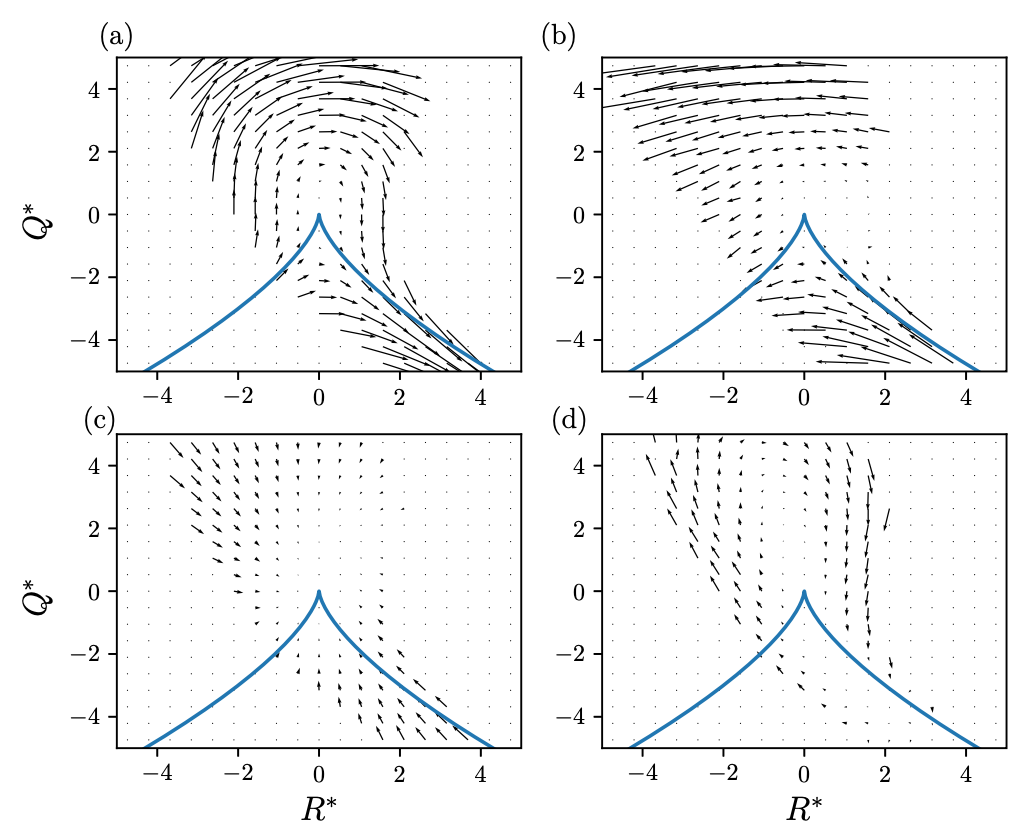
\includegraphics[width=0.75\textwidth]{LagrangianDeformationModels/figs/tian_qr_cmt.png}
    \caption{The ground truth conditional mean tangents (CMTs) in the $Q\text{-}R$ phase plane arising from (a) Restricted Euler (b) deviatoric pressure Hessian (c) viscous (d) sum of all terms. Taken from Tian et.al, \color{red}{TODO generate this figure.}}
    \label{fig:gt_qr_cmt}
\end{figure}

In the case of incompressible turbulence we can write the formal (nonlocal) solution for the deviatoric pressure Hessian as a spatial integral \cite{ohkitani1995} in the Eularian frame
\begin{equation} \label{eq:nonlocal_solution}
    H_{ij}({\bm x}) = \iiint \frac{\delta_{ij} - \hat{r_i}\hat{r_j}}{2\pi r^3}Q({\bm x} + {\bm r})d{\bm r}
\end{equation}
where $Q = \frac{1}{2}\tr(A^2)$, and ${\bm x}\in\mathbb{R}^3$.

The challenge then, is to obtain an approximation of this integral using only local information.


\subsection{Tensor Basis Neural Network}
Following Lawson \& Dawson \cite{lawson2015}, an expansion of the integral in eq(\ref{eq:nonlocal_solution}) is proposed, first as a Taylor series expansion in $Q({\bm x}+{\bm r})$
\begin{equation}
  \hat{H} = \sum_{m,n = 0}^\infty \alpha_{mn}S^mW^n
\end{equation}
where
\begin{equation}
  S = \frac{1}{2}(A + A^T) \qquad W = \frac{1}{2}(A - A^T)
\end{equation}

Finally we can reduce from an infinite sum using Cayley-Hamilton, and expand via the tensor basis\cite{zheng1993},\cite{pope1975}
\begin{equation}
  \hat{H} = \sum_{n=1}^{10} g^{(n)}(\lambda_1, \dots, \lambda_5)T^{(n)}
\end{equation}
with $g^{(n)}$ scalar functions of the invariants
\begin{equation}
  \lambda_1 = \tr(S^2) \quad \lambda_2 = \tr(W^2) \quad \lambda_3 = \tr(S^3) \quad \lambda_4 = \tr(W^2S) \quad \lambda_5 = \tr(W^2S^2)
\end{equation}
and the tensor basis given by:
\begin{align} \label{eq:tb_start}
  &T^{(1)} = S &T^{(2)} &= SW-WS\\
  &T^{(3)} = S^2 - \frac{1}{3}I \cdot \tr(S^2) &T^{(4)} &= W^2 - \frac{1}{3}I \cdot \tr(W^2)\\
  &T^{(5)} = WS^2 - S^2W &T^{(6)} &= W^2S + SW^2 - \frac{2}{3}I \cdot \tr(SW^2)\\
  &T^{(7)} = WSW^2-W^2SW &T^{(8)} &= SWS^2 - S^2WS\\
  &T^{(9)} = W^2S^2 + S^2W^2 - \frac{2}{3}I \cdot \tr(S^2W^2) &T^{(10)} &= WS^2W^2 - W^2S^2W \label{eq:tb_end}
\end{align}
This formulation reduces the challenge to finding the functions of known scalars, i.e., learning the $g^{(n)}$'s as shown in fig(\ref{fig:tbnn_architecture}).

This network architecture ensures the output tensor $\hat{H}$ is symmetric, traceless, and the network itself is rotationally and Galilean invariant. A technical note, since we are using the $L_2$ loss, $\hat{H}$ is only an approximation to the mean deviatoric pressure Hessian if the statistics of the pressure Hessian are normal. As we expect turbulent statistics to be non-Gaussian, the choice of loss is driven more by mathematical convenience. 

\begin{figure}
    \centering
    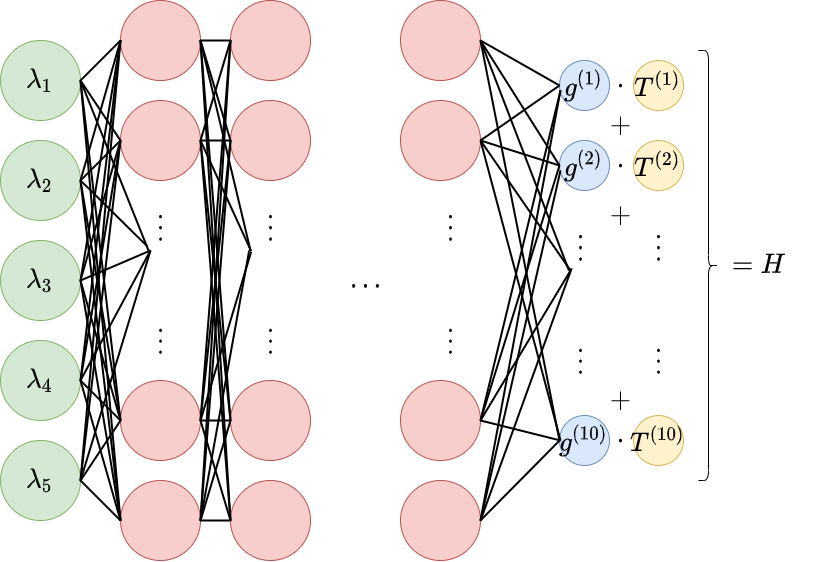
\includegraphics[width=0.5\linewidth]{InterpretableML/figs/tbnn.png}
    \caption{The architecture of the TBNN. The invariants and tensor basis elements are calculated from each sample of the VGT, the invariants are then used as input to a fully connected network, and the resulting $g^{(i)}$ multiply the corresponding tensor basis elements $T^{(i)}$, before summing into the prediction $\hat{H}$}
    \label{fig:tbnn_architecture}
\end{figure}

Tian et.al \cite{tian2021} showed ability to train the network, and demonstrated state-of-the-art performance on a variety of relevant physical metrics: eigenvector alignments, $Q\text{-}R$ conditional mean tangents (CMTs), and \textit{a posteriori} tests evolving an initially Gaussian field to fully developed turbulence as evidenced by characteristic teardrop-shaped $Q\text{-}R$ probability distributions (PDFs).

\begin{figure}
    \centering
    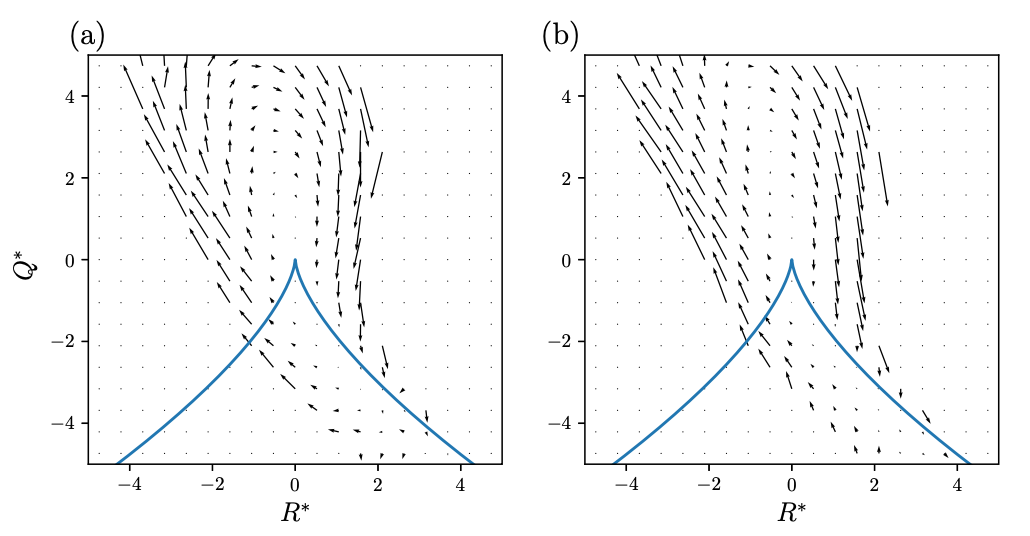
\includegraphics[width=0.85\linewidth]{LagrangianDeformationModels/figs/tian_tbnn_qrcmt.png}
    \caption{Results from Tian et.al\cite{tian2021} showing $Q\text{-}R$ CMTs from (a) DNS data and (b) trained TBNN}
    \label{fig:tian_qrcmt}
\end{figure}

\subsection{Recent Deformation of Gaussian Fields}

Johnson and Meneveau \cite{johnson2016} introduced the RDGF model following a long line of postulating that the deviatoric part of the pressure Hessian could be locally modeled using information of the time history of the deformation tensor \cite{chertkov1999},\cite{chevillard2006lagrangian},\cite{chevillard2008modeling}. 

Chertkov et.al's Tetrad Model \cite{chertkov1999}, attempted to capture this deformation directly by following a small fluid element approximated by four Lagrangian particles, initialized in an isotropic configuration. This model avoided the finite time singularity resulting from using only the restricted Euler term\cite{cantwell1992}. Attempts to fuse this low-dimensional model of a fluid element with data-driven methods for prediction of the coarse-grained VGT are ongoing \cite{hyett2021machine},\cite{hyett2020machine}. Chevillard \& Meneveau used the same isotropic Lagrangian upstream condition as in the Tetrad Model when developing their Recent Fluid Deformation (RFD) model. Most recently, Johnson \& Meneveau enriched the approximation of the upstream condition to that of a Gaussian field using high fidelity direct numerical simulation (DNS) data\cite{wan2016johns}.

RDGF models the conditional average of the (full) pressure Hessian tensor as:
\begin{equation}
    \hat{P}_{ij} = \frac{\partial y_k}{\partial x_i} \frac{\partial^2 p}{\partial y_k\partial y_l} \frac{\partial y_l}{\partial x_j} = D^{-1}_{ki} \tilde{P}_{kl} D^{-1}_{lj},
\end{equation}
where $\tilde{P}$ is the pressure Hessian tensor/matrix evaluated along the Lagrangian trajectory upstream in time. The deformation tensor, defined as a sensitivity  of a particle observed at the position $x$ at the moment of time $t$ to its initial position $y$ at the previous moment of time,
\begin{equation}
    D_{ij} = \frac{\partial x_i}{\partial y_j},
\end{equation}
evolves according to 
\begin{equation}\label{eq:Deformation-tensor}
    \frac{d D_{ij}}{dt} = A_{ik} D_{kj}, \quad \text{ with }  D_{ij}(0) = \delta_{ij},
\end{equation}
assuming isotropic initial condition (without loss of generality for sufficiently far removed upstream times). Solution of Eq.~(\ref{eq:Deformation-tensor}) is defined via the time-ordered exponential
\begin{equation}
    D(t) = \text{Texp}\left(\int\limits_0^t dt' A(t')\right) = \lim_{N\to \infty} \prod_{i = 0}^N \left( e^{A(t_i)\Delta t} \right),
\end{equation}
where %the product is the left product, and 
$t_i=i \Delta t$ and $\Delta t= t/N$. %t_0 = 0, t_N=t$ and $\Delta t=$. 
If we take $N=1$ and set $\Delta t$ to be the smallest temporal scale of turbulence (also called the Kolmogorov, or viscous scale) we arrive at %the leading order term, we get 
the RDGF approximation for the deformation tensor
\begin{equation}
    \hat{D}(x,t) = \exp\left( A(x,t) \Delta t \right) \approx D(\Delta t).
\end{equation}

All that is left is to determine the upstream pressure Hessian $\tilde P$. The RDGF model uses a Gaussian field closure for $\tilde P$,

\begin{equation} \label{eq:rdgf_upstream}
    \hat{\tilde{P}}_{ij} = \frac{1}{3} \tilde{P}_{kk} \delta_{ij} + \langle \tilde{P}^{(d)}_{ij} | A 
    \rangle_{\text{Gaussian}}
\end{equation}
where $\langle \tilde{P}^{(d)} | A\rangle_{Gaussian}$ is the mean deviatoric pressure Hessian in a Gaussian field, found by Wilczek \& Meneveau\cite{wilczek2014pressure}. Using the notation of the tensor basis [Eqs.~(\ref{eq:tb_start}-\ref{eq:tb_end})], they found
\begin{equation}
    \langle \tilde{P}^{(d)}_{ij} | A \rangle_{\text{Gaussian}} = \gamma T^{(2)} + \alpha T^{(3)} + \beta T^{(4)}
\end{equation}
with the value of the coefficients found from a mix of theoretical and numerical experiments
\begin{equation} \label{eq:rdgf_coefs}
    \alpha = -\frac{2}{7}, \quad \beta=-\frac{2}{5}, \quad \gamma \approx 0.08.
\end{equation}

Introducing the deformed Gaussian field approximation
\begin{equation}
    \hat{G}_{ij} := \hat{D}_{mi}^{-1}\langle \tilde{P}_{mn}^{(d)} | A \rangle_{\text{Gaussian}} \hat{D}_{nj}^{-1},
\end{equation}
and a short-time approximation to the inverse of the left Cauchy-Green tensor
\begin{equation}
    \hat{C}^{-1}_{ij} = \hat{D}^{-1}_{ki}\hat{D}^{-1}_{kj}
\end{equation}
We enforce the prediction in Eq.~(\ref{eq:rdgf_upstream}) to have the correct trace, and arrive at the following RDGF prediction for the component of the pressure Hessian conditioned to the VGT
\begin{equation}
    \hat{P}_{ij} = 2Q \frac{\hat{C}^{-1}_{ij}}{\hat{C}^{-1}_{kk}} + \hat{G}_{ij} - \frac{\hat{C}^{-1}_{ij}}{\hat{C}^{-1}_{kk}}\hat{G}_{ll}.
\end{equation}